% Options for packages loaded elsewhere
\PassOptionsToPackage{unicode}{hyperref}
\PassOptionsToPackage{hyphens}{url}
\documentclass[
]{article}
\usepackage{xcolor}
\usepackage{textgreek}
\usepackage{amsmath,amssymb}
\setcounter{secnumdepth}{-\maxdimen} % remove section numbering
\usepackage{iftex}
\ifPDFTeX
  \usepackage[T1]{fontenc}
  \usepackage[utf8]{inputenc}
  \usepackage{textcomp} % provide euro and other symbols
\else % if luatex or xetex
  \usepackage{unicode-math} % this also loads fontspec
  \defaultfontfeatures{Scale=MatchLowercase}
  \defaultfontfeatures[\rmfamily]{Ligatures=TeX,Scale=1}
\fi
\usepackage{lmodern}
\ifPDFTeX\else
  % xetex/luatex font selection
\fi
% Use upquote if available, for straight quotes in verbatim environments
\IfFileExists{upquote.sty}{\usepackage{upquote}}{}
\IfFileExists{microtype.sty}{% use microtype if available
  \usepackage[]{microtype}
  \UseMicrotypeSet[protrusion]{basicmath} % disable protrusion for tt fonts
}{}
\makeatletter
\@ifundefined{KOMAClassName}{% if non-KOMA class
  \IfFileExists{parskip.sty}{%
    \usepackage{parskip}
  }{% else
    \setlength{\parindent}{0pt}
    \setlength{\parskip}{6pt plus 2pt minus 1pt}}
}{% if KOMA class
  \KOMAoptions{parskip=half}}
\makeatother
\usepackage{longtable,booktabs,array}
\usepackage{calc} % for calculating minipage widths
% Correct order of tables after \paragraph or \subparagraph
\usepackage{etoolbox}
\makeatletter
\patchcmd\longtable{\par}{\if@noskipsec\mbox{}\fi\par}{}{}
\makeatother
% Allow footnotes in longtable head/foot
\IfFileExists{footnotehyper.sty}{\usepackage{footnotehyper}}{\usepackage{footnote}}
\makesavenoteenv{longtable}
\usepackage{graphicx}
\makeatletter
\newsavebox\pandoc@box
\newcommand*\pandocbounded[1]{% scales image to fit in text height/width
  \sbox\pandoc@box{#1}%
  \Gscale@div\@tempa{\textheight}{\dimexpr\ht\pandoc@box+\dp\pandoc@box\relax}%
  \Gscale@div\@tempb{\linewidth}{\wd\pandoc@box}%
  \ifdim\@tempb\p@<\@tempa\p@\let\@tempa\@tempb\fi% select the smaller of both
  \ifdim\@tempa\p@<\p@\scalebox{\@tempa}{\usebox\pandoc@box}%
  \else\usebox{\pandoc@box}%
  \fi%
}
% Set default figure placement to htbp
\def\fps@figure{htbp}
\makeatother
\setlength{\emergencystretch}{3em} % prevent overfull lines
\providecommand{\tightlist}{%
  \setlength{\itemsep}{0pt}\setlength{\parskip}{0pt}}
\usepackage{bookmark}
\IfFileExists{xurl.sty}{\usepackage{xurl}}{} % add URL line breaks if available
\urlstyle{same}
\hypersetup{
  hidelinks,
  pdfcreator={LaTeX via pandoc}}

\author{}
\date{}

\begin{document}

{FISICA}

{}

\section{\texorpdfstring{{Unità }{di
misura}}{Unità di misura}}\label{h.l5wfwwv3cbxn}

\subsection{\texorpdfstring{{S.I.}}{S.I.}}\label{h.hw5gyoas23ps}

{Sistema Internazionale, comprende le seguenti unità fondamentali:}

{}

\begin{longtable}[]{@{}lll@{}}
\toprule\noalign{}
\endhead
\bottomrule\noalign{}
\endlastfoot
{Nome} & {Unità} & {Simbolo} \\
{Lunghezza} & {Metro} & {m} \\
{Massa} & {Chilogrammo} & {kg} \\
{Intervallo di tempo} & {Secondo} & {s} \\
{Intensità di corrente elettrica} & {Ampere} & {A} \\
{Temperatura} & {Kelvin} & {K} \\
{Intensità luminosa} & {Candela} & {cd} \\
{Quantità di materia} & {Mole} & {mol} \\
\end{longtable}

{}

{Da queste unità base è possibile ricavare unità derivate.}

{}

{~Esempio: Kg -\textgreater{} g}

{}

{Il SI è }{coerente}{, cioè il prodotto o il rapporto di due unità da
un'altra unità del SI, }{assoluto}{, le unità }{non}{~}{cambiano in base
al luogo o al momento, e }{decimale}{, cioè multipli e sottomultipli
corrispondono alle potenze di 10.}

\subsection{\texorpdfstring{{Analisi
dimensionale}}{Analisi dimensionale}}\label{h.4b09ywiqwmvv}

{Con il }{SI è}{~possibile ricavare nuove unità, dalla combinazione di
quelle fondamentali possiamo fare l'analisi }{dimensionale }{(dimensione
= ``natura delle grandezze fisiche coinvolte'') delle equazioni delle
leggi fisiche che incontreremo.}

{}

\section{\texorpdfstring{{Calcolo
vettoriale}}{Calcolo vettoriale}}\label{h.93p8g45f8wyi}

{Con alcune grandezze un solo numero non basta per rappresentarle, per
questo si usa il calcolo vettoriale.}

{\pandocbounded{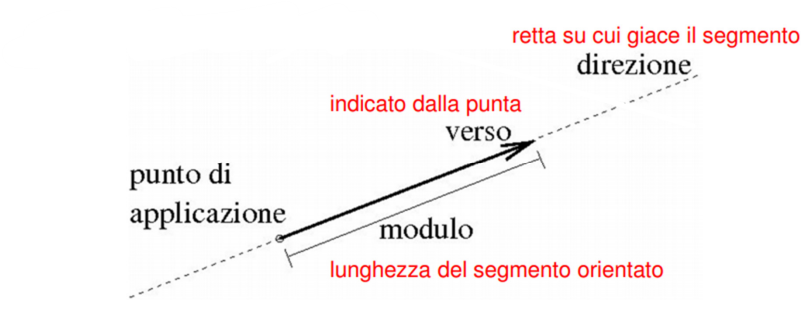
\includegraphics[keepaspectratio]{images/image61.png}}}

{Tramite il teorema di Pitagora,seno e coseno possiamo trovare le
componenti di un vettore.}

{\pandocbounded{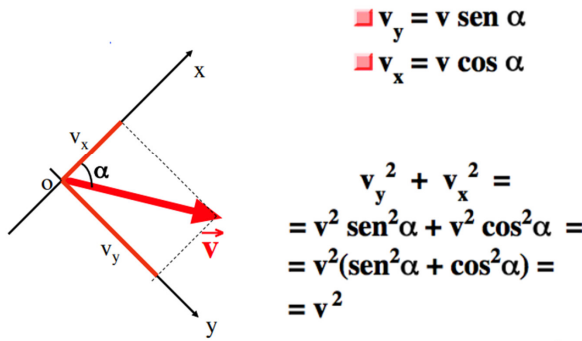
\includegraphics[keepaspectratio]{images/image65.png}}}

{Si decide se usare sen/cos in base all'asse utilizzato (in questo caso
X)}

{}

{Il modulo:}

\pandocbounded{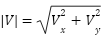
\includegraphics[keepaspectratio]{images/image1.png}}

\subsection{\texorpdfstring{{Somma}}{Somma}}\label{h.beivh3hgpdth}

{È possibile sommare i vettori con il metodo del parallelogramma o
sommando le componenti.}

{\pandocbounded{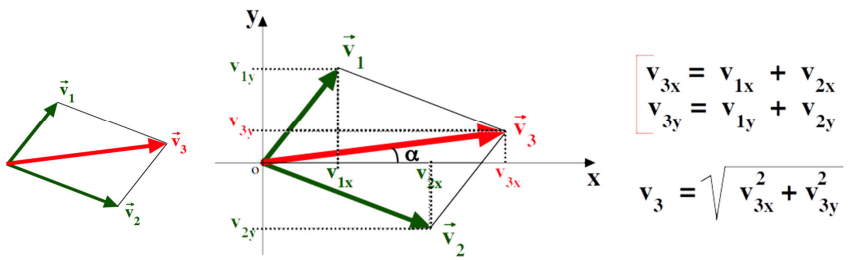
\includegraphics[keepaspectratio]{images/image59.png}}}

{Con parallelogramma}

{\pandocbounded{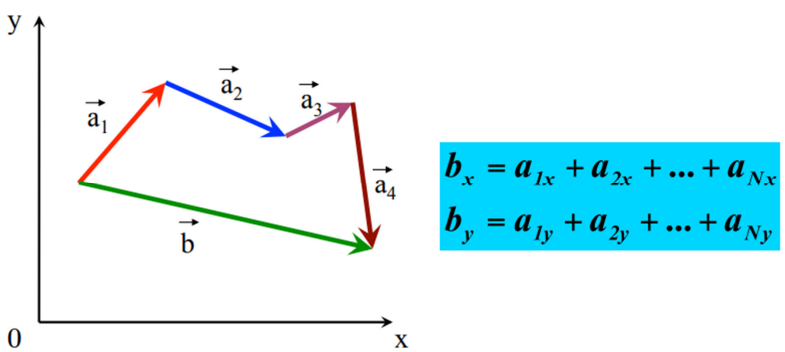
\includegraphics[keepaspectratio]{images/image62.png}}}

{Sommando componenti}

{}

\subsection{\texorpdfstring{{Differenza}}{Differenza}}\label{h.qqcggqhskpvf}

{La differenza si fa invertendo il verso del vettore da sottrarre o
sottraendo fra loro le componenti.}

{\pandocbounded{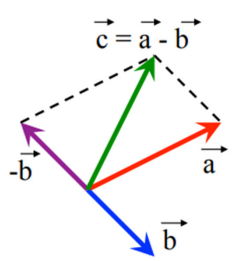
\includegraphics[keepaspectratio]{images/image67.png}}}

{Modo grafico}

{\pandocbounded{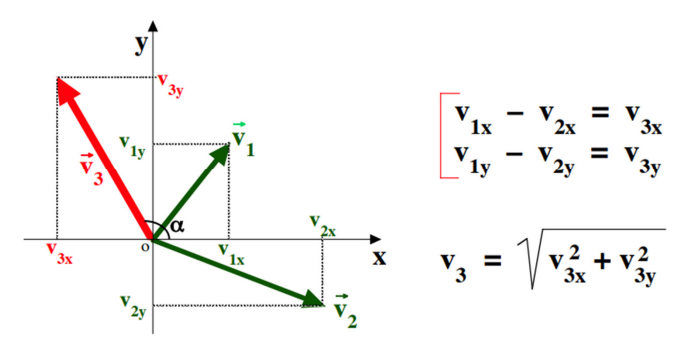
\includegraphics[keepaspectratio]{images/image70.png}}}

{Sottraendo componenti}

{}

\subsection{\texorpdfstring{{Prodotto
scalare}}{Prodotto scalare}}\label{h.ccgpw5h6cpxl}

{Il risultato }{non}{~è un vettore, ma uno scalare (numero) che
rappresenta i loro moduli quando i due vettori sono paralleli.}

{\pandocbounded{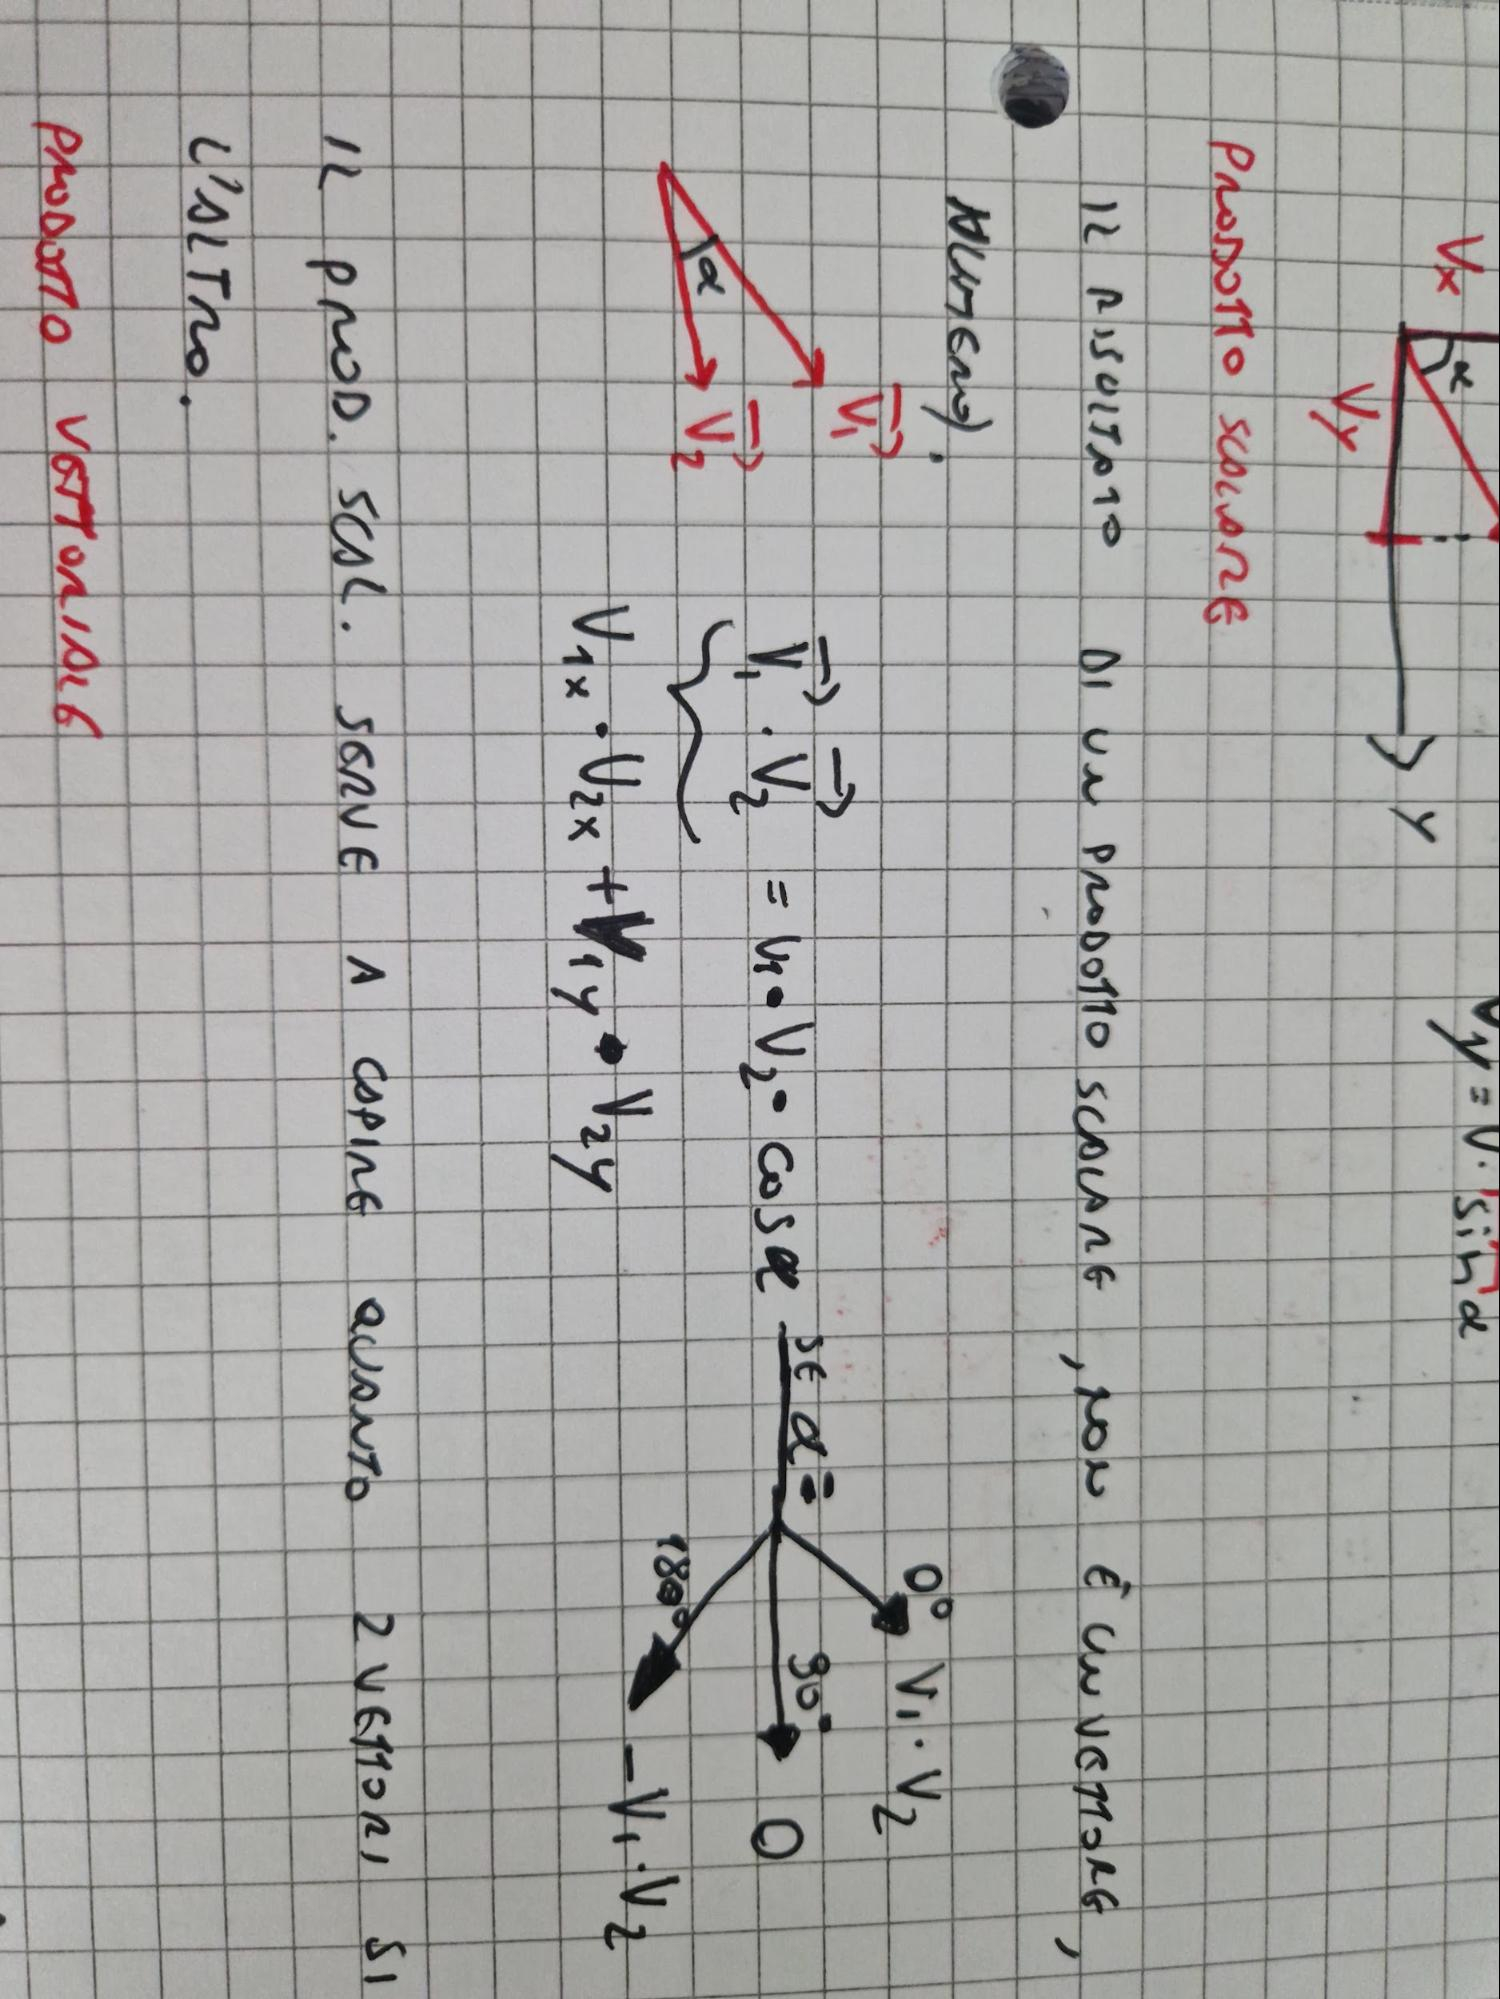
\includegraphics[keepaspectratio]{images/image63.jpg}}}

\subsection{\texorpdfstring{{Prodotto
vettoriale}}{Prodotto vettoriale}}\label{h.5nbhpw85z5fw}

{Il risultato è un vettore, si usa la regola della mano }{destra}{.}

{}

{\pandocbounded{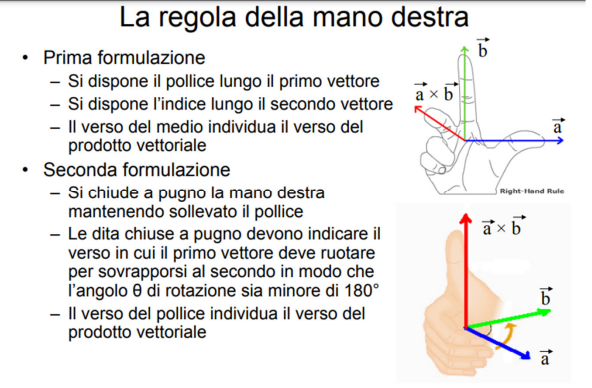
\includegraphics[keepaspectratio]{images/image64.png}}}

{Il prodotto vettoriale tra due vettori a e b nello spazio è definito
da:}

\pandocbounded{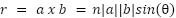
\includegraphics[keepaspectratio]{images/image2.png}}

{\pandocbounded{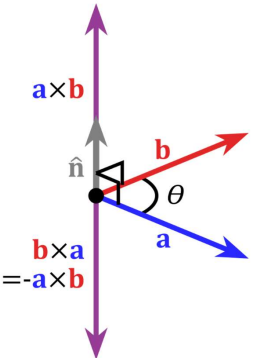
\includegraphics[keepaspectratio]{images/image76.png}}}

{o}

\pandocbounded{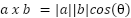
\includegraphics[keepaspectratio]{images/image3.png}}

{}

\subsubsection{\texorpdfstring{{Proprietà}}{Proprietà}}\label{h.rbyya54pej89}

\begin{itemize}
\tightlist
\item
  {Il modulo del prodotto vettoriale è pari all'area del parallelogramma
  individuato dai due vettori;}
\item
  {Il prodotto vettoriale è nullo se i due vettori sono paralleli}
\item
  {Il prodotto vettoriale gode della }{proprietà anticommutativa (b x a
  = -a x b)}{.}
\end{itemize}

\section{\texorpdfstring{{Trigonometria}}{Trigonometria}}\label{h.ue79vjagpw72}

{\pandocbounded{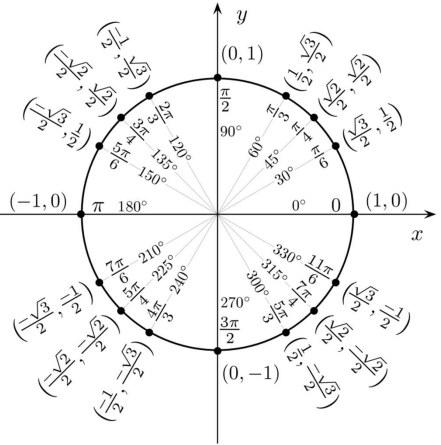
\includegraphics[keepaspectratio]{images/image78.png}}}

{(}{cos}{,}{sin}{) ← Legenda}

{}

{Il }{coseno}{~}{è la parte che è parallela
all}{\textquotesingle{}}{asse X}{, il }{seno}{~}{è la parte che è
parallela all'}{asse Y}{.}

\subsubsection{\texorpdfstring{{Formula duplicazione
angoli}}{Formula duplicazione angoli}}\label{h.dho1p7xfsfbd}

{Esprime il valore di un angolo doppio in funzione del valore di un
angolo semplice.}

{}

{sin(2$(x, y, \theta)$) = }{2sin}{($(x, y, \theta)$)cos($(x, y, \theta)$)}

{~cos(2$(x, y, \theta)$) = cos\^{}2($(x, y, \theta)$) - sin\^{}2($(x, y, \theta)$)}

{}

\section{\texorpdfstring{{Moto}}{Moto}}\label{h.imao6m7ejpzy}

\subsection{\texorpdfstring{{Unidimensionale}}{Unidimensionale}}\label{h.gedl4e75hk77}

{Il moto unidimensionale si riferisce a un movimento che avviene lungo
una singola direzione, ad esempio lungo una retta.}

\subsubsection{\texorpdfstring{{Velocità}}{Velocità}}\label{h.u8baxmf7pyck}

{Formula velocità}{:
}\pandocbounded{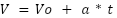
\includegraphics[keepaspectratio]{images/image4.png}}{(dove
a = costante di gravità e Vo = velocità al momento)}

{↑}

{Cambiamento di velocità }{più}{~accelerazione per il tempo}

{}

{Formula velocità istantanea}{:
}\pandocbounded{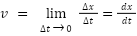
\includegraphics[keepaspectratio]{images/image5.png}}{~}{(velocità
in un dato istante di tempo)}

{↑}

{Derivata della posizione rispetto al tempo}

\subsubsection{\texorpdfstring{{Accelerazione}}{Accelerazione}}\label{h.n808ronr2ejg}

{Variazione }{di velocità:}

{}

\pandocbounded{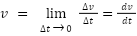
\includegraphics[keepaspectratio]{images/image6.png}}

{}

{Accelerazione costante, 3 casi:}

{}

\begin{enumerate}
\tightlist
\item
  \pandocbounded{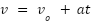
\includegraphics[keepaspectratio]{images/image7.png}}
\end{enumerate}

{\pandocbounded{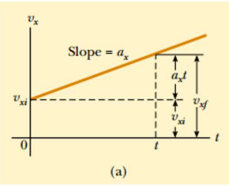
\includegraphics[keepaspectratio]{images/image77.png}}}

\begin{enumerate}
\setcounter{enumi}{1}
\tightlist
\item
  \pandocbounded{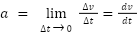
\includegraphics[keepaspectratio]{images/image8.png}}
\end{enumerate}

{\pandocbounded{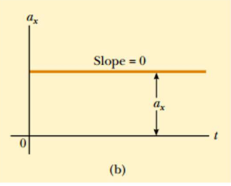
\includegraphics[keepaspectratio]{images/image69.png}}}

\begin{enumerate}
\setcounter{enumi}{2}
\tightlist
\item
  \pandocbounded{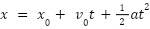
\includegraphics[keepaspectratio]{images/image9.png}}{~(}{x}{o}{~=
  punto di partenza, }{v}{o}{~= velocità al momento, }{t}{~= tempo
  impiegato}{).}
\end{enumerate}

{\pandocbounded{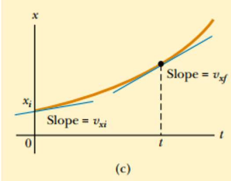
\includegraphics[keepaspectratio]{images/image73.png}}}

{}

{}

{}

\subsection{\texorpdfstring{{Su più
dimensioni}}{Su più dimensioni}}\label{h.cskrlavz2cw2}

{Se consideriamo il moto in più dimensioni accelerazione e velocità
possono anche non essere parallele; usando la scomposizione dei vettori
possiamo scomporre il moto in componenti per ciascun asse e trattare
queste in modo indipendente. }

{}

{\pandocbounded{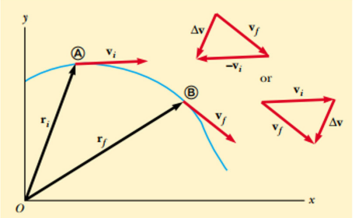
\includegraphics[keepaspectratio]{images/image71.png}}}

{}

{In un moto arbitrario sono presenti due tipi di accelerazioni:}

{}

\begin{itemize}
\tightlist
\item
  {Tangenziale}{: indica la variazione della velocità di un oggetto
  lungo la direzione tangente alla sua traiettoria (come la velocità di
  un oggetto cambia in termini di modulo o direzione nel corso del
  tempo);}
\item
  {Centripeta}{: accelerazione diretta verso il centro di una
  traiettoria circolare. Questa accelerazione è necessaria per mantenere
  un oggetto su una traiettoria circolare e dipende dalla velocità e dal
  raggio della curva}
\end{itemize}

\section{\texorpdfstring{{Forze}}{Forze}}\label{h.molkyw15qzlx}

{Unità di misura: }{Newton (N)}

\subsection{\texorpdfstring{{Leggi di
Newton}}{Leggi di Newton}}\label{h.mflpysdw6sz5}

{Legge universale:}

\pandocbounded{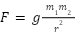
\includegraphics[keepaspectratio]{images/image10.png}}

\subsubsection{\texorpdfstring{{Prima}}{Prima}}\label{h.2ewv6w5bdn6d}

{Se la somma di tutte le forze applicate a un corpo è 0 allora non
cambierà il suo stato di quiete o di moto.}

\subsubsection{\texorpdfstring{{Seconda}}{Seconda}}\label{h.45xg1f6o44w}

{L'accelerazione di un oggetto è direttamente proporzionale alla somma
delle forze agenti su di esso e inversamente proporzionale alla sua
MASSA.}

\pandocbounded{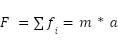
\includegraphics[keepaspectratio]{images/image11.png}}

\subsubsection{\texorpdfstring{{Terza}}{Terza}}\label{h.sv2r3n5ivjor}

{Se due oggetti interagiscono, la forza
}\pandocbounded{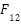
\includegraphics[keepaspectratio]{images/image12.png}}{~esercitata
dall\textquotesingle oggetto 1 sull\textquotesingle oggetto 2 è uguale
in grandezza e opposta in direzione }{alla}{~forza
}\pandocbounded{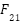
\includegraphics[keepaspectratio]{images/image13.png}}{~esercitata
dall\textquotesingle oggetto 2 sull\textquotesingle oggetto 1.}

{}

\pandocbounded{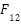
\includegraphics[keepaspectratio]{images/image12.png}}{~=
}\pandocbounded{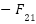
\includegraphics[keepaspectratio]{images/image14.png}}

\subsection{\texorpdfstring{{Attrito}}{Attrito}}\label{h.x94iyldv7377}

{Quando un corpo è posto su di una superficie vi è attrito fra i due. La
forza di attrito si oppone al moto ed è proporzionale alla forza normale
alla superficie. Il corpo non si muove finché non viene superato
l'attrito statico poi rallenta secondo l'attrito dinamico.}

\subsection{\texorpdfstring{{Conservativa}}{Conservativa}}\label{h.zd4ikqvvff4b}

{Una forza è conservativa se: }

{}

\begin{itemize}
\tightlist
\item
  {Il lavoro che fa su una particella che si muove tra due punti
  qualsiasi è indipendente dal percorso fatto dalla particella;}
\end{itemize}

{}

\begin{itemize}
\tightlist
\item
  {Il lavoro fatto da una forza conservativa su una particella che si
  muove attraverso un percorso chiuso è zero. ~}
\end{itemize}

{}

\section{\texorpdfstring{{Energia e
Lavoro}}{Energia e Lavoro}}\label{h.zh05bw4n6uco}

{Lavoro: }{energia trasferita }{a un oggetto quando questo viene messo
in movimento.}

{Si calcola con il prodotto scalare fra la forza applicata e il suo
vettore spostamento:}

{}

\pandocbounded{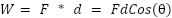
\includegraphics[keepaspectratio]{images/image15.png}}{~}{(d
-\textgreater{} vettore percorso}{)}

{oppure (se non sono costanti)}

\pandocbounded{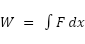
\includegraphics[keepaspectratio]{images/image16.png}}

{Il segno dipende dalla variazione di velocità e si misura in Joule
{[}J{]}.}

\subsection{\texorpdfstring{{Legge di
Hooke}}{Legge di Hooke}}\label{h.eii8b14m63js}

{Prendendo come esempio una molla:}

{Se }{non }{si deforma (se siamo in regime elastico) spostandola dalla
sua posizione di equilibrio una molla }{eserciterà}{~una forza
proporzionale ed opposta allo spostamento:}

{}

{F = -kx}

\subsection{\texorpdfstring{{Energia
cinetica}}{Energia cinetica}}\label{h.6zmenjm9d3fv}

{Se consideriamo il lavoro fatto su una particella esso equivale al
cambiamento della sua energia cinetica:}

\pandocbounded{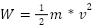
\includegraphics[keepaspectratio]{images/image17.png}}

{}

\subsection{\texorpdfstring{{Potenza}}{Potenza}}\label{h.n211wdn7wjw7}

{La potenza media è un lavoro {[}w{]} applicato per un certo tempo.}

{}

\pandocbounded{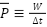
\includegraphics[keepaspectratio]{images/image18.png}}

{La potenza istantanea:}

{}

\pandocbounded{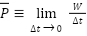
\includegraphics[keepaspectratio]{images/image19.png}}

\pandocbounded{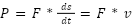
\includegraphics[keepaspectratio]{images/image20.png}}{~{[}Watt{]}}

\subsection{\texorpdfstring{{Energia
potenziale}}{Energia potenziale}}\label{h.f7fdtba8iraa}

{Nei }{sistemi conservativi}{~è il lavoro che il sistema potrebbe fare
su un oggetto, es: sistemi gravitazionali.}

{}

\pandocbounded{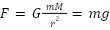
\includegraphics[keepaspectratio]{images/image21.png}}

{}

{Lavoro fatto da una forza gravitazionale se un corpo cade da una
altezza}\pandocbounded{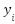
\includegraphics[keepaspectratio]{images/image22.png}}{~fino
ad
}\pandocbounded{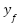
\includegraphics[keepaspectratio]{images/image23.png}}{~:
}

{}

\pandocbounded{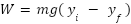
\includegraphics[keepaspectratio]{images/image24.png}}

{}

{}

{quindi possiamo scrivere:}

{}

\pandocbounded{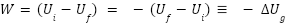
\includegraphics[keepaspectratio]{images/image25.png}}

{dove
}\pandocbounded{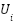
\includegraphics[keepaspectratio]{images/image26.png}}{:
energia pot. iniziale }

{e}

{~}\pandocbounded{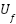
\includegraphics[keepaspectratio]{images/image27.png}}{:
energia pot. finale}

{e}

\pandocbounded{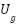
\includegraphics[keepaspectratio]{images/image28.png}}{:
energia gravitazionale}

{}

{In un sistema elastico abbiamo:}

\pandocbounded{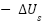
\includegraphics[keepaspectratio]{images/image29.png}}

{}

\subsection{\texorpdfstring{{Energia
meccanica}}{Energia meccanica}}\label{h.von70sgtz3mh}

{Per TUTTI i sistemi conservativi possiamo definire una energia
meccanica totale
}\pandocbounded{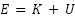
\includegraphics[keepaspectratio]{images/image30.png}}{~che
è costante in assenza di altre forze agenti sul corpo.}

{}

\subsection{\texorpdfstring{{Pendolo}}{Pendolo}}\label{h.1oediyvcos6u}

{Un pendolo è una massa attaccata a un filo leggero e di lunghezza
costante.}

{Se vogliamo calcolare il periodo per piccole oscillazioni:}

{}

\pandocbounded{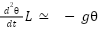
\includegraphics[keepaspectratio]{images/image31.png}}

{e otteniamo}

\pandocbounded{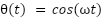
\includegraphics[keepaspectratio]{images/image32.png}}

{}

{}

\section{\texorpdfstring{{Quantità di
moto}}{Quantità di moto}}\label{h.ra024frm88jc}

{Detto anche momento, è un vettore definito come:
}\pandocbounded{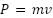
\includegraphics[keepaspectratio]{images/image33.png}}{~(massa
* velocità)}

{Il momento è costante e si conserva. }

\subsection{\texorpdfstring{{Urti}}{Urti}}\label{h.7cxlqym634h6}

{Nel caso di un urto fra particelle esistono due casi limite: negli urti
elastici l'energia cinetica è conservata e in quelli anelastici si
perde.}

\subsubsection{\texorpdfstring{{Legge di
Noether}}{Legge di Noether}}\label{h.bts61n3qizrd}

{Ad ogni SIMMETRIA corrisponde una quantità conservata}

{}

{Per la conservazione del momento:}

\pandocbounded{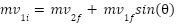
\includegraphics[keepaspectratio]{images/image34.png}}{~}{applicata
in Y}

{o}

\pandocbounded{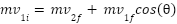
\includegraphics[keepaspectratio]{images/image35.png}}{~}{applicata
in X}

{Andando a misurare l'angolo con cui vengono deviate le traiettorie si
ottiene il rapporto delle velocità.}

{}

\section{\texorpdfstring{{Centro di
massa}}{Centro di massa}}\label{h.j1d37uwj89ku}

{Le coordinate del CENTRO DI MASSA di un sistema di particelle sono date
dalla media pesata delle coordinate delle particelle con la loro massa.}

{}

\pandocbounded{\includegraphics[keepaspectratio]{images/image36.png}}

{oppure con gli infinitesimi}

\pandocbounded{\includegraphics[keepaspectratio]{images/image37.png}}

{}

{Derivando la prima formula:}

\pandocbounded{\includegraphics[keepaspectratio]{images/image38.png}}

{}

{Applicando la 3° legge di Newton:}

\pandocbounded{\includegraphics[keepaspectratio]{images/image39.png}}

{}

{Il centro di massa di un sistema di particelle di massa totale M si
muove come si muoverebbe una equivalente massa M sotto
l\textquotesingle influenza della risultante delle forze esterne agenti
sul sistema.}

{}

{}

{}

{}

{}

\subsection{\texorpdfstring{{Spinta}}{Spinta}}\label{h.2wyy8turwf1v}

\pandocbounded{\includegraphics[keepaspectratio]{images/image40.png}}

{}

{}

\section{\texorpdfstring{{Analisi
errori}}{Analisi errori}}\label{h.a8pn2fciw7bd}

{Ogni volta che facciamo una misura il valore che otteniamo è affetto da
una incertezza ovvero da un errore inevitabile.}

{}

{Esistono due regole per riportare in modo corretto i dati
sperimentali:}

{}

\begin{enumerate}
\tightlist
\item
  {Le incertezze vanno arrotondate ad UNA cifra significativa;}
\end{enumerate}

{}

\begin{enumerate}
\setcounter{enumi}{1}
\tightlist
\item
  {L'ultima cifra significativa di una misura deve essere dello stesso
  ordine di grandezza dell'incertezza.}
\end{enumerate}

{}

{Questo vuol dire che scriveremo: }

{1.2 +/- 0.5 e non 1.2+/- 0.}{48912667}{~}

{E NON }

{1.2}{353456}{~+/- 0.5}

{}

\subsection{\texorpdfstring{{Incertezza}}{Incertezza}}\label{h.cuh8tfbvoudd}

{Può essere espressa come incertezza relativa (precisione):}

{}

\pandocbounded{\includegraphics[keepaspectratio]{images/image41.png}}

{}

{o anche}

{}

{Incertezza percentuale:}

\pandocbounded{\includegraphics[keepaspectratio]{images/image42.png}}

\subsection{\texorpdfstring{{Errori casuali e
sistematici}}{Errori casuali e sistematici}}\label{h.1c2bijdupztb}

{\pandocbounded{\includegraphics[keepaspectratio]{images/image80.png}}}

{}

{}

{}

\section{\texorpdfstring{{Elettronica}}{Elettronica}}\label{h.1h99sf20oto}

\subsection{\texorpdfstring{{Legge di
Ohm}}{Legge di Ohm}}\label{h.av8cgi8cjzv2}

{}

{V = RI }

{(resistività * cariche al secondo)}

{}

{NON è sempre valida. I conduttori cambiano la propria
}{resistività}{~con la temperatura (e quindi possono essere usati come
sensori di temperatura) mentre nei semiconduttori la legge non è
valida.}

{}

{La legge completa è:}

\pandocbounded{\includegraphics[keepaspectratio]{images/image43.png}}

{a e
}\pandocbounded{\includegraphics[keepaspectratio]{images/image44.png}}{sono
costanti}

{e}

\pandocbounded{\includegraphics[keepaspectratio]{images/image45.png}}

\subsection{\texorpdfstring{{Serie e
parallelo}}{Serie e parallelo}}\label{h.md78lgo1tlqz}

{Si dice che elementi elettrici sono in SERIE quando sono attraversati
dalla stessa corrente:}

{\pandocbounded{\includegraphics[keepaspectratio]{images/image72.png}}}

\pandocbounded{\includegraphics[keepaspectratio]{images/image46.png}}

{}

{Mentre sono detti IN PARALLELO quando ai loro capi è applicata la
stessa differenza di potenziale:}

{\pandocbounded{\includegraphics[keepaspectratio]{images/image66.png}}}

\pandocbounded{\includegraphics[keepaspectratio]{images/image47.png}}

{La capacità si trova:}

\pandocbounded{\includegraphics[keepaspectratio]{images/image48.png}}{~}{dove
la Q = carica}

{}

{Il Wattaggio:}

\pandocbounded{\includegraphics[keepaspectratio]{images/image49.png}}

\subsection{\texorpdfstring{{Leggi di
Kirchhoff}}{Leggi di Kirchhoff}}\label{h.fkx934jjylz7}

{Iniziamo dicendo che un }{nodo}{~è un incrocio di più conduttori o rami
di un circuito; una maglia è un percorso chiuso in un circuito.}

\subsubsection{\texorpdfstring{{1°
legge}}{1° legge}}\label{h.glck7lbk4vz7}

{La somma delle correnti che affluiscono a un NODO è = 0 }

\subsubsection{\texorpdfstring{{2°
legge}}{2° legge}}\label{h.qsbb4njka1cc}

{La somma delle differenze di potenziale lungo una MAGLIA è = 0}

{}

{Quindi se in un circuito abbiamo una batteria da 7 Volt la somma di
tutte le resistenze deve essere 7 Volt totali.}

{}

{}

{}

{}

\subsection{\texorpdfstring{{Teorema di
Thévenin}}{Teorema di Thévenin}}\label{h.mj1oeeb3s2p3}

{Una qualunque rete lineare può essere modellizzata da due dei suoi nodi
A e B come la serie di un generatore di tensione
}\pandocbounded{\includegraphics[keepaspectratio]{images/image50.png}}{~e
una resistenza
}\pandocbounded{\includegraphics[keepaspectratio]{images/image51.png}}{.}

{}

{~}\pandocbounded{\includegraphics[keepaspectratio]{images/image50.png}}{~è
uguale alla tensione presente ai capi A e B aperti mentre
}\pandocbounded{\includegraphics[keepaspectratio]{images/image51.png}}{~si
ottiene cortocircuitando tutti i generatori di tensione e interrompendo
tutti i generatori di corrente.}

{\pandocbounded{\includegraphics[keepaspectratio]{images/image60.png}}}

\subsection{\texorpdfstring{{Teorema di
Norton}}{Teorema di Norton}}\label{h.n26dau9t3e4i}

{Una qualunque rete lineare può essere modellizzata tra due dei suoi
nodi A e B come il parallelo di un generatore di corrente
}\pandocbounded{\includegraphics[keepaspectratio]{images/image52.png}}{e
una resistenza
}\pandocbounded{\includegraphics[keepaspectratio]{images/image53.png}}{.
}

{}

\pandocbounded{\includegraphics[keepaspectratio]{images/image52.png}}{~}{è
uguale alla corrente che scorre fra i capi A e B cortocircuitati mentre
}{~}\pandocbounded{\includegraphics[keepaspectratio]{images/image53.png}}{~}{si
ottiene cortocircuitando tutti i generatori di tensione e interrompendo
tutti i generatori di corrente.}

{}

{\pandocbounded{\includegraphics[keepaspectratio]{images/image75.png}}}

{}

{}

{}

{}

\section{\texorpdfstring{{Analisi
statistica}}{Analisi statistica}}\label{h.c3c6175ywqd3}

{La media di N misure è definita:}

\pandocbounded{\includegraphics[keepaspectratio]{images/image54.png}}{~}

{(somma di tutti i valori / il numero di misure fatte)}

{}

{La media è un estimatore statistico, questi ``tools'' si utilizzano per
avere misure migliori, un altro è la deviazione }{quaratica}{~media
(RMS), che viene usata per rappresentare l'incertezza del singolo dato:}

{\pandocbounded{\includegraphics[keepaspectratio]{images/image79.png}}}

{}

{media degli scarti al quadrato}

{}

{}

{La media pesata per N misure ripetute:}

{\pandocbounded{\includegraphics[keepaspectratio]{images/image68.png}}}

{si usa per andare a pesare di più certi valori nella media}

{}

{}

\subsection{\texorpdfstring{{Teorema del limite
centrale}}{Teorema del limite centrale}}\label{h.6wr8eccyska4}

{Il teorema del limite centrale afferma che:}

{~la somma o la media di un gran numero di variabili aleatorie
indipendenti e dotate della stessa distribuzione è
}{distribuito}{~secondo la distribuzione di Gauss indipendentemente
dalla distribuzione soggiacente. }

{}

{Questo significa che la distribuzione di alcune statistiche come per
esempio la media del campione }{diventa}{~nota anche se non sappiamo
nulla a proposito della forma della distribuzione della popolazione da
cui i campioni sono stati tratti.}

{}

{}

{}

{}

{}

\section{\texorpdfstring{{Circuiti}}{Circuiti}}\label{h.8lv14blsfsi4}

\subsection{\texorpdfstring{{RL}}{RL}}\label{h.gw1tnriwzbpt}

{Un circuito RL è un circuito che contiene una resistenza (R) e una
bobina (L). I circuiti RL possono essere utilizzati per filtrare
segnali, generare impulsi, stabilizzare tensioni, e gestire il
comportamento temporale dei segnali.}

{}

{La resistenza è un componente passivo che limita il flusso di corrente
nel circuito. Misurata in ohm ($\Omega$), la resistenza dissipa energia sotto
forma di calore. Nel circuito RL, la resistenza influisce sulla caduta
di tensione e sulla dissipazione di energia.}

{}

{Una bobina è un componente che immagazzina energia sotto forma di campo
magnetico quando attraversata da una corrente. La bobina ha
un\textquotesingle induttanza (L) misurata in henry (H).
L\textquotesingle induttanza determina la capacità della bobina di
opporsi a variazioni rapide di corrente e di immagazzinare energia.}

{}

{}

{Tramite la seguente formula si trova il tempo di costante:}

{t=L/R}

{}

{}

\subsection{\texorpdfstring{{LC}}{LC}}\label{h.nstmyfwqsvh8}

{Un circuito LC è un tipo di circuito che comprende un induttanza (L) e
un condensatore (C). Questi circuiti sfruttano le proprietà di
immagazzinamento di energia di entrambi i componenti per creare
oscillazioni e risonanze.}

{}

{L\textquotesingle induttanza è un componente che immagazzina energia
sotto forma di campo magnetico quando attraversato da una corrente.
Viene misurata in henry (H). L\textquotesingle induttanza in un circuito
LC influisce sulla velocità di variazione della corrente e sulla
frequenza di oscillazione del circuito.}

{}

{Un condensatore è un componente che immagazzina energia sotto forma di
campo elettrico tra le sue piastre quando viene applicata una differenza
di potenziale. Viene misurato in farad (F). Il condensatore in un
circuito LC influisce sulla capacità di immagazzinare carica e sulla
frequenza di oscillazione del circuito.}

{}

{}

{Energia accumulata dal condensatore:}

{}

\pandocbounded{\includegraphics[keepaspectratio]{images/image55.png}}

{}

{Equazione oscillatore armonico:}

{}

{q(t) =
}\pandocbounded{\includegraphics[keepaspectratio]{images/image56.png}}\pandocbounded{\includegraphics[keepaspectratio]{images/image57.png}}

{}

{}

\section{\texorpdfstring{{Amplificatori
Operazionali}}{Amplificatori Operazionali}}\label{h.iwci826bwx9c}

{\pandocbounded{\includegraphics[keepaspectratio]{images/image81.png}}}

{}

{Il modello ideale di amplificatore operazionale implica che la
differenza di tensione fra le uscite sia sempre uguale a zero quando
siamo in presenza di una retro reazione.}

{Il circuito più semplice che possiamo realizzare è quello di un buffer
non invertente. In questo circuito la tensione di ingresso viene
riportata in uscita con guadagno uno, l'importanza di questo circuito
sta nel fatto che in data l\textquotesingle{} impedenza infinita di
ingresso dell\textquotesingle amplificatore operazionale questo circuito
ci permette di misurare tensioni in un sistema senza
}{perturbarlo}{~comportandosi come buffer.}

{}

\subsection{\texorpdfstring{{Non
invertente}}{Non invertente}}\label{h.w68fnrvcgkdh}

{Un amplificatore non invertente è un tipo di configurazione di
amplificazione utilizzando un amplificatore operazionale in cui il
segnale in ingresso viene amplificato senza essere invertito in fase
nell\textquotesingle uscita. Questa configurazione è ampiamente
utilizzata in applicazioni in cui è necessario amplificare un segnale
senza cambiarne la polarità.}

{}

{P}{revede }{due resistenze}{, una collegata
}{all\textquotesingle ingresso invertente}{~dell\textquotesingle op-amp
a una tensione di riferimento (solitamente la massa o un punto di
tensione stabile), e l\textquotesingle altra collegata
}{tra}{~}{l\textquotesingle uscita dell\textquotesingle op-amp e
l\textquotesingle ingresso non invertente}{. L\textquotesingle ingresso
del segnale da amplificare viene collegato all\textquotesingle ingresso
non invertente.}

{}

{\pandocbounded{\includegraphics[keepaspectratio]{images/image74.png}}}

{}

{Il }{guadagno }{si trova con:}

\pandocbounded{\includegraphics[keepaspectratio]{images/image58.png}}

{R1}{~{[}R}{F}{{]}}{~-\textgreater{} collegata
all\textquotesingle ingresso / R2 }{~{[}R}{2}{{]}}{~-\textgreater{}
collegata all'uscita}

{}

{}

{}

{}

{}

\subsection{\texorpdfstring{{Comparatore con
isteresi}}{Comparatore con isteresi}}\label{h.caqcz1f70il2}

{Un circuito comparatore dotato di isteresi è un tipo di circuito che
utilizza un amplificatore operazionale per confrontare due tensioni di
ingresso e fornire un\textquotesingle uscita che cambia in modo definito
e stabile tra due soglie specifiche.}

{}

{Questo tipo di circuito è utilizzato per rilevare la transizione di
tensione tra due stati, introducendo una regione di isteresi che
impedisce commutazioni indesiderate dell\textquotesingle uscita in
presenza di segnali rumorosi o fluttuanti vicino alle soglie di
commutazione.}

{}

{Un esempio è il comparatore Schmitt Trigger.}

{}

{}

{}

{}

{}

{}

{}

\section{\texorpdfstring{{DOMANDE SLIDES (da
fare)}}{DOMANDE SLIDES (da fare)}}\label{h.2fdulleeuzgg}

{}

\end{document}
